\documentclass{article}

%% Language and font encodings
\usepackage[utf8x]{inputenc}
\usepackage{polski}
\usepackage{hyperref}
\usepackage{dirtytalk}
\usepackage{listings}
\usepackage{graphicx}
\usepackage{float}
\usepackage{caption}

%% Useful packages
\usepackage{amsmath}
\usepackage{amsthm}
\usepackage{amsfonts}
\usepackage[colorinlistoftodos]{todonotes}

\title{ROB Laboratorium 2 - sprawozdanie}
\author{Artur M. Brodzki}

\begin{document}
	\maketitle
	
	\section{Wstęp} \label{sec:intro}
	Celem projektu jest porównanie skuteczności klasyfikacji maści kart optymalnym klasyfikatorem Bayesa, w zależności od metody estymacji rozkładów prawdopodobieństwa. Pliki z wykorzystanym kodem zostały przesłane razem z niniejszym sprawozdaniem. W ramach laboratorium zaimplementowano następujące funkcje wymagane w treści polecenia:
	\begin{itemize}
		\item para\_indep.m i pdf\_indep.m, służące do estymacji rozkładu prawdopodobieństwa metodą niezależnych rozkładów Gaussa
		\item para\_multi.m i pdf\_multi.m, służące do estymacji rozkładu prawdopodobieństwa metodą wielowymiarowego rozkładu Gaussa
		\item para\_parzen.m i pdf\_parzen.m, służące do estymacji rozkładu prawdopodobieństwa metodą okna Parzena
		\item reduce.m, funkcja wybierająca ze zbioru danych pewien jego podzbiór w sposób losowy
	\end{itemize}
	Oprócz powyższych, zaimplementowano kilka dodatkowych funkcji pomocniczych pozwalających na wygodne generowanie wymaganych wyników:
	\begin{itemize}
		\item delete\_extremes.m, funkcja usuwająca ze zbioru danych obserwacje odstające. Opisana szczegółowo w rozdziale \ref{sec:outliers}. 
		\item rename\_classes.m, funkcja zmieniająca 4 etykiety maści kart na 8 etykiet danych, zgodnie z treścią zadania. 
		\item rob2\_ercf.m, funkcja obliczająca skuteczność klasyfikatora Bayesa dla zadanych danych wszystkimi trzema metodami estymacji rozkładu prawdopodobieństwa. Dla klasyfikatora Parzena wykonuje kilka eksperymentów, dla kilku zadanych wartości szerokości okna. Szczegółowy opis funkcji znajduje się w sekcji \ref{sec:experiments}. 
	\end{itemize}
	W pliku mainscript.m znajdują się jedynie wywołania funkcji rob2\_ercf i pomocniczych, pozwalające na wygenerowanie na standardowe wyjście wymaganych wyników. 
	
	\section{Analiza zbioru uczącego} \label{sec:set_analysis}
	
	\subsection{Usuwanie obserwacji odstających} \label{sec:outliers}
	Zalecenia zawarte w pliku mainscript.m proponują znalezienie obserwacji odstających poprzez "obejrzenie" wartości maksymalnych, minimalnych oraz median parametrów dla zadanych zbiorów, a także skorzystanie z dwuwymiarowych wykresów generowanych za pomocą funkcji plot2features. Jest to metoda analizy "na oko" (nawet jeśli z użyciem median i wartości ekstremalnych) i niesie ryzyko pominięcia niektórych obserwacji odstających; nie dałaby się również zastosować do większych zbiorów danych. Mimo to obejrzyjmy kilka takich wykresów. Rysunki \ref{fig:train-23}-\ref{fig:train2-56} przedstawiają rzuty zbioru treningowego train.txt na różne pary cech. 
	\begin{figure} \centering 
		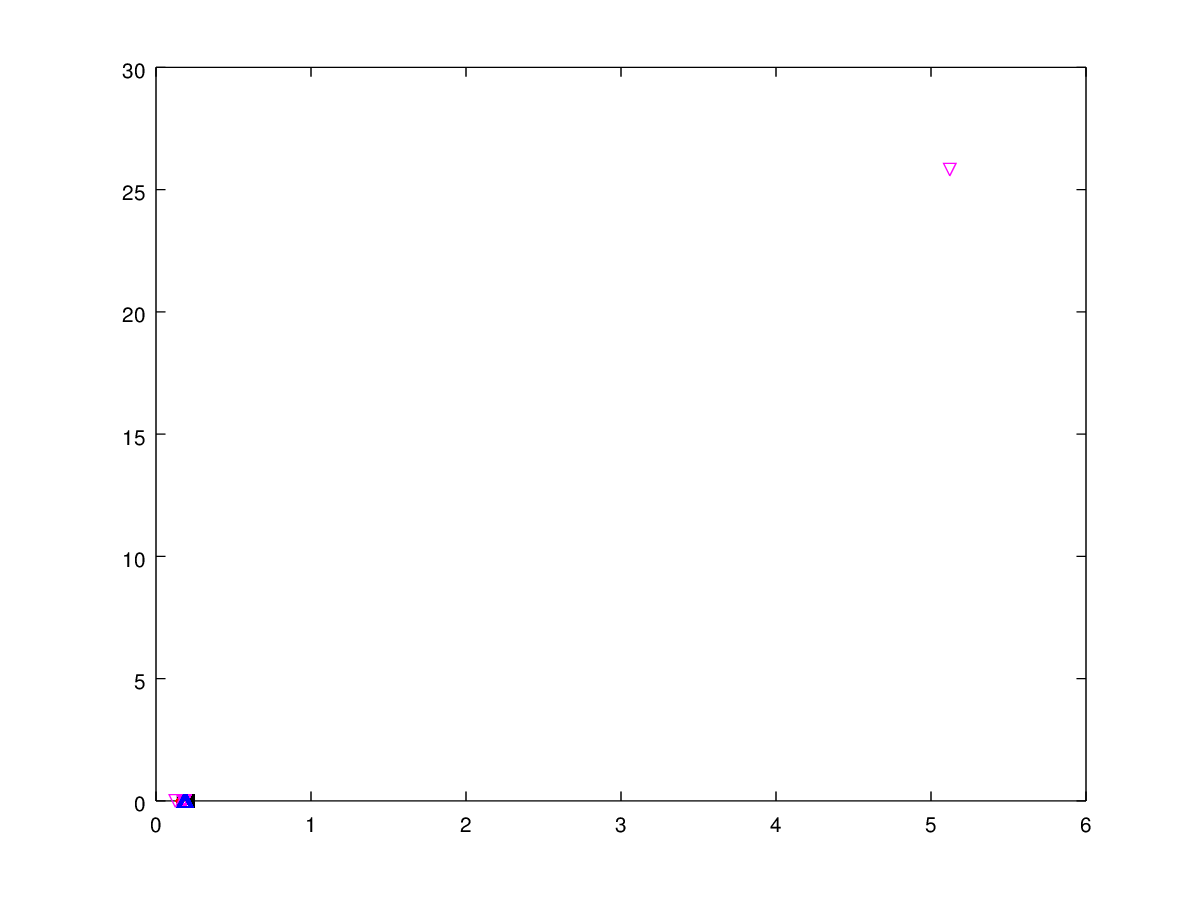
\includegraphics[height = 7cm]{plot-train-2-3.png}
		\caption[First figure]{Rzut zbioru treningowego na cechy 2,3. }
		\label{fig:train-23}
	\end{figure}
    \begin{figure} \centering 
    	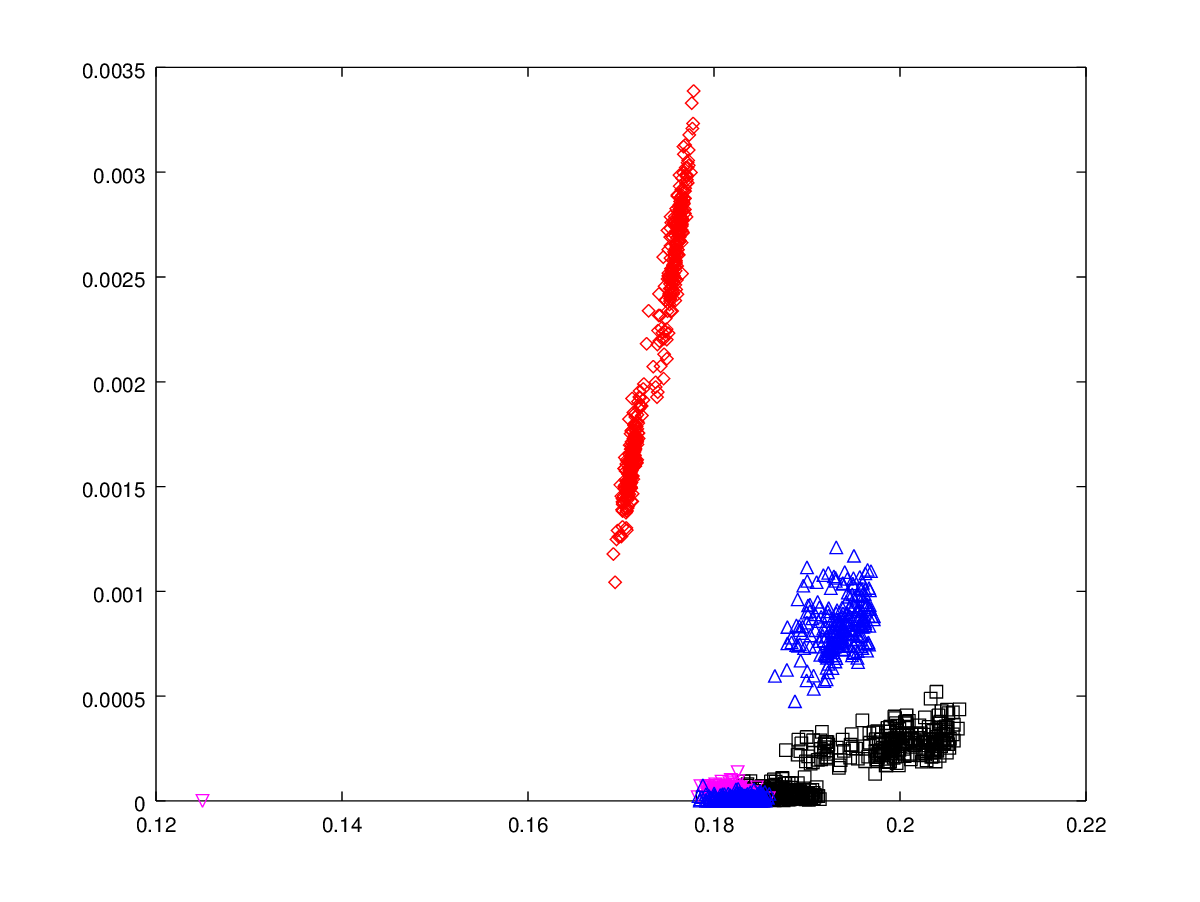
\includegraphics[height = 7cm]{plot-train2-2-3.png}
    	\caption{Rzut zbioru treningowego na cechy 2,3 po usunięciu punktu 186. }
    	\label{fig:train2-23}
    \end{figure}
	\begin{figure} \centering 
		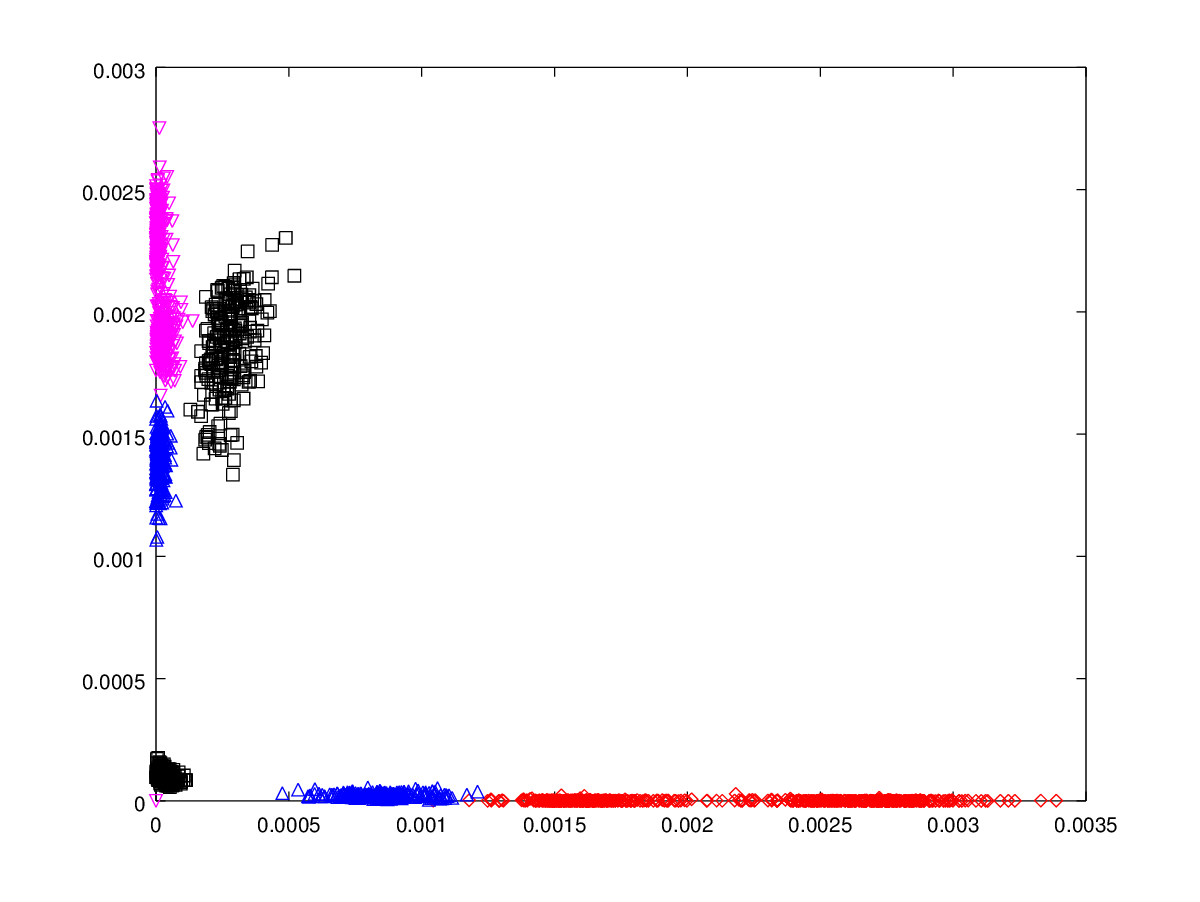
\includegraphics[height = 7cm]{plot-train2-3-4.png}
		\caption{Rzut zbioru treningowego na cechy 3,4 po usunięciu punktu 186. }
		\label{fig:train2:34}
	\end{figure}
	\begin{figure} \centering 
		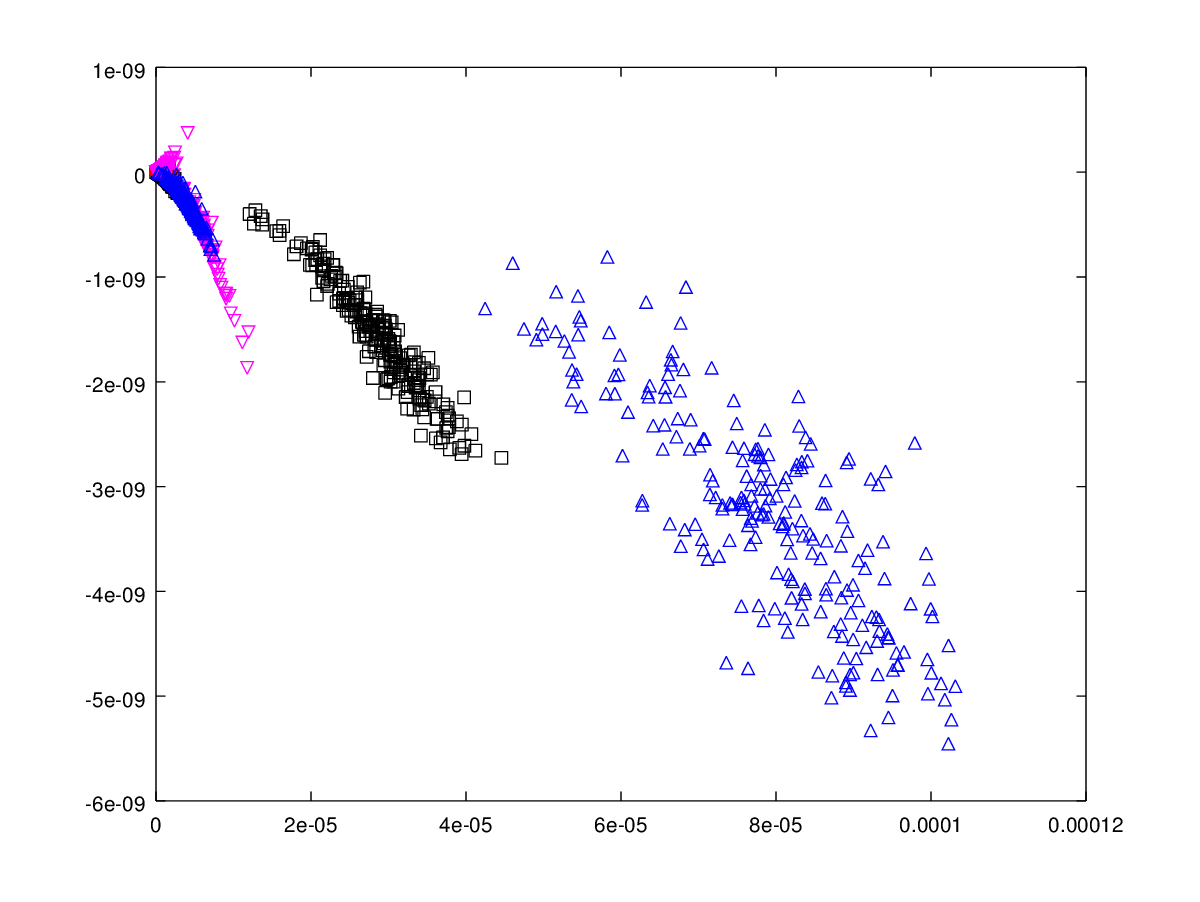
\includegraphics[height = 7cm]{plot-train2-5-6.png}
		\caption{Rzut zbioru treningowego na cechy 5,6 po usunięciu punktu 186.  }
		\label{fig:train2-56}
	\end{figure}
	Wyraźnie widoczna jest odstająca obserwacja na Rysunku \ref{fig:train-23}. Jest to punkt 186; po jego usunięciu, widoczna jest również - zwłaszcza na rysunku \ref{fig:train2-23} - obserwacja odstająca w pobliżu współrzędnych (0,0). Jest to punkt 642. On również został usunięty z danych. Dalsza analiza, w tym z wykorzystaniem median oraz wartości ekstremalnych, nie wykazała istnienia innych obserwacji odstających. 
	
	Jak wspomniano, metoda szukania wartości odstających "na oko", jakkolwiek kusząca swoją prostotą, jest inherentnie wadliwa. Do znajdowania wartości odstających można jednak wykorzystać funkcję pdf\_multi.m. Ponieważ punkty odstające z definicji znajdują się daleko od pozostałych punktów w zbiorze, można założyć, że ich estymowane prawdopodobieństwo wystąpienia będzie bardzo niskie. Rozsądnym wydaje się założenie, że prawdopodobieństwo punktu w zbiorze danych dane jest wielowymiarowym rozkładem normalnym. Zatem za wartość odstająca możemy uznać punkt, którego estymowana gęstość prawdopodobieństwa jest niższa od zadanego progu. Ponieważ zarówno w zbiorze uczącym jak i testowym mamy po 1824 punkty, przyjęto próg równy 0.0001. Do usuwania z danych wartości odstających tą metodą stworzono funkcję delete\_extremes.m. Funkcja przyjmuje jako pierwszy parametr zbiór danych do analizy, a jako drugi - próg gęstości prawdopodobieństwa. Usuwane punkty są wypisywane na standardowe wyjście. 
	
	Okazuje się, że lista znalezionych wartości odstających zależy od sposobu etykietowania maści kart. Gdy dane są - zgodnie ze swoją naturą - etykietowane przez 8 klas, znalezione wartości odstające są te same, co metodą "na oko": 186 i 642. Ich estymowana gęstość prawdopodobieństwa jest rzędu $10^{-76}$ oraz $10^{-70}$, zatem nie może być wątpliwości co do ich natury. W przypadku, gdy używamy tylko 4 klas, dodatkowo znajdowane są jeszcze trzy punkty: 40 ($10^{-42}$), 42 ($10^{-21}$) i 512 ($10^{-16}$). Nie są one widoczne na wykresach gołym okiem, ze względu na bardzo niewielką skalę zmienności względem sąsiednich klas (rys. \ref{fig:train2-45-autoscale}). Ich natura jako obserwacji odstających uwidacznia się po obejrzeniu wykresów w odpowiednim powiększeniu - rys. \ref{fig:train2-45}. 
	\begin{figure} \centering 
		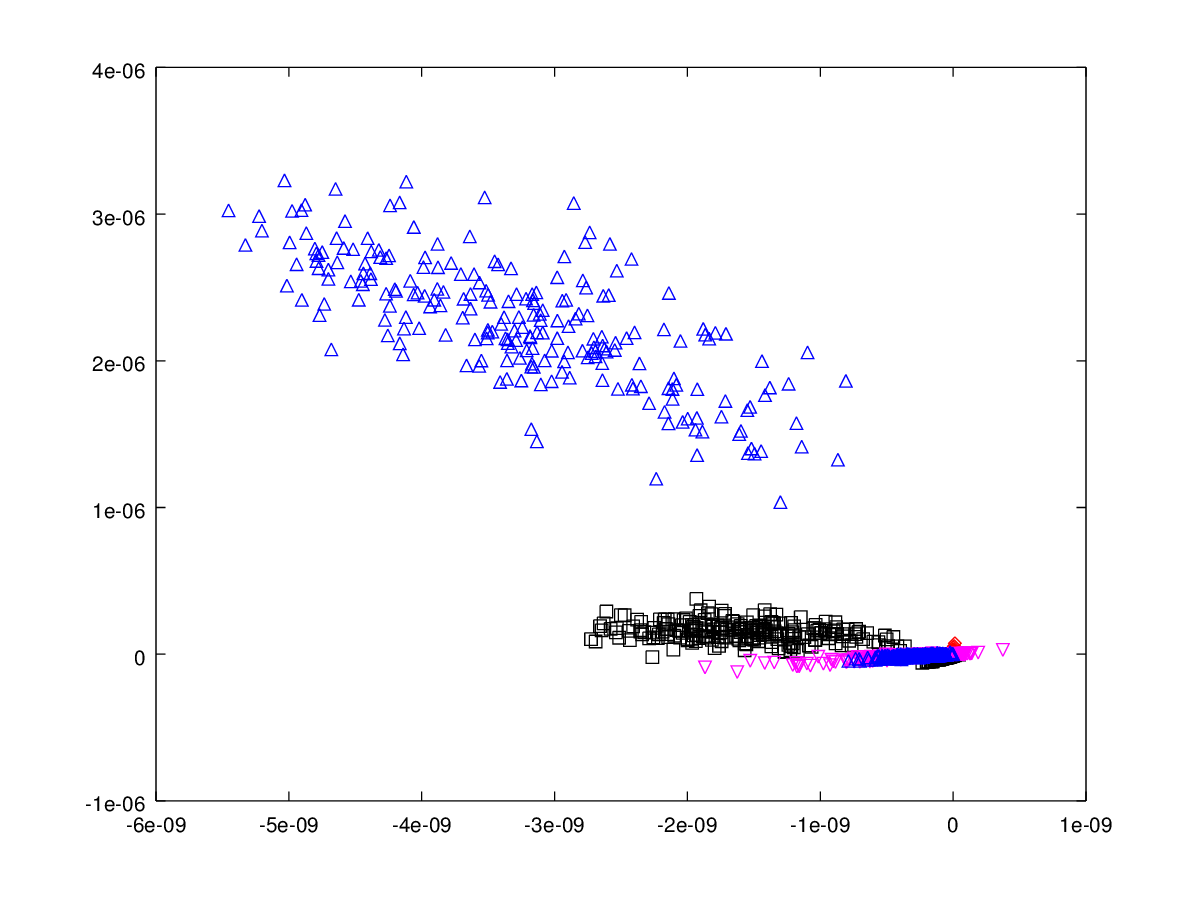
\includegraphics[height = 7cm]{plot-train2-67-autoscale.png}
		\caption{Rzut zbioru treningowego na cechy 6,7. Widoczne skupienie punktów klasy czerwonej na niewielkim obszarze, w pobliżu współrzędnych (0,0). }
		\label{fig:train2-45-autoscale}
	\end{figure}
    \begin{figure} \centering 
    	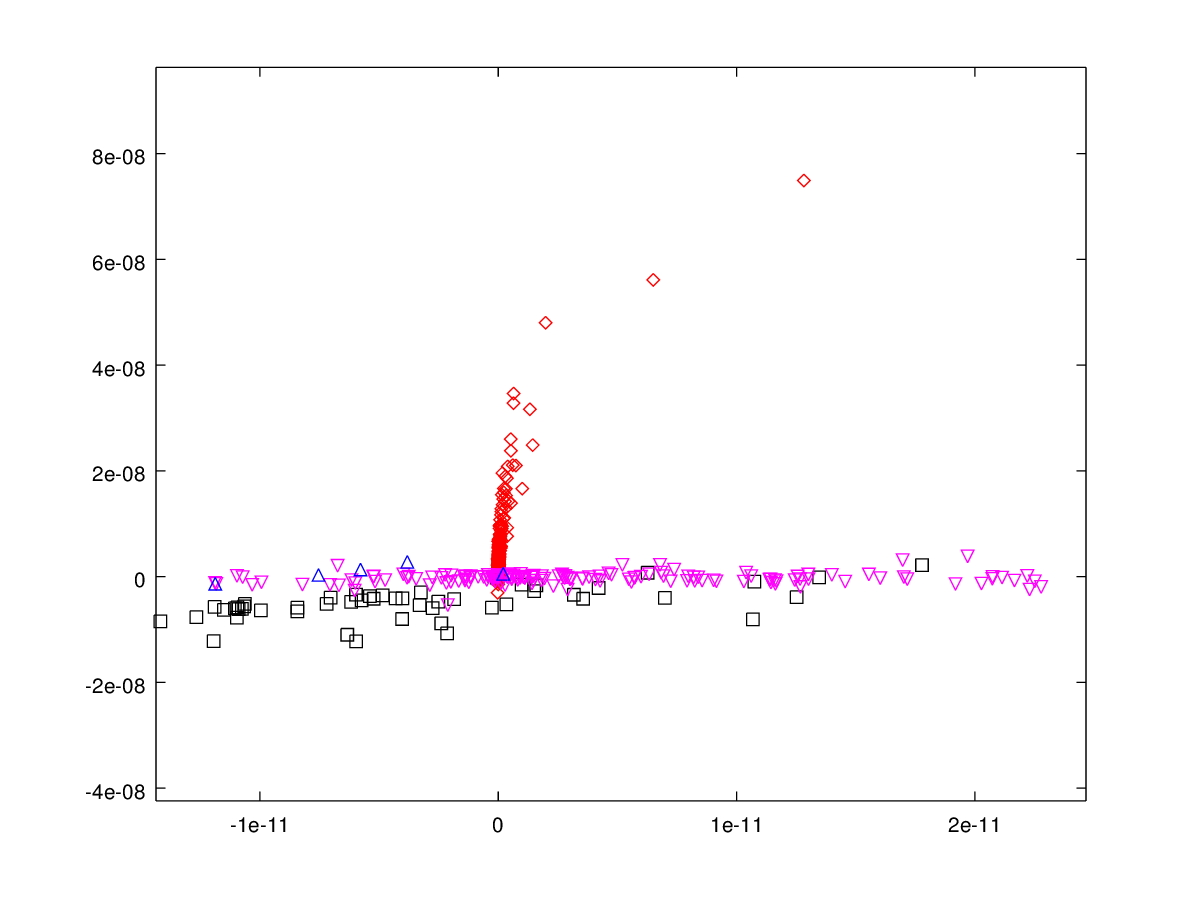
\includegraphics[height = 7cm]{plot-train2-67.png}
    	\caption{Rzut zbioru treningowego na cechy 6,7 - powiększenie zbioru punktów czerwonych. Widoczne trzy obserwacje odstające (punkty kolejno 512, 42 i 40) w prawej górnej części - w przeciwieństwie do pozostałych punktów, nie układają się w prostej wąskiej linii. }
    	\label{fig:train2-45}
    \end{figure}
	Ponieważ w większości eksperymentów wykonywanych w ramach laboratorium stosuje się 8 etykiet klas, zasadniczo usunięto ze zbioru danych punkty 186 i 642. Jednak w tych eksperymentach, w których wykorzystywane są tylko 4 klasy, usunięto również punkty 40, 42 i 512. 
	
	Pozostaje jeszcze wybór dwóch cech do klasyfikacji. Na podstawie oglądania wykresów zdecydowano o wyborze cech 3 i 4. Jak widać na rysunku \ref{fig:train2:34}, w tej konfiguracji poszczególne klasy są względnie dobrze od siebie oddzielone (nie zachodzą na siebie zbyt mocno), co daje perspektywę na dobre wyniki klasyfikacji. 
	
	\section{Eksperymenty} \label{sec:experiments}
	
	Wykonano następujące eksperymenty:
	\begin{enumerate}
		\item Klasyfikacja na klasyfikatorze uczonym pełnym zbiorem treningowym i testowanym na pełnym zbiorze testowym (prawdopodobieństwa apriori takie same dla każdej klasy):
		\begin{enumerate}
			\item Dla 8 klas i szerokości okna Parzena kolejno 0.00025, 0.0005, 0.00075, 0.001, 0.00125, 0.0015, 0.00175, 0.002. 
			\item Dla 4 klas i szerokości okna Parzena kolejno 0.00025, 0.0005, 0.00075, 0.001, 0.00125, 0.0015, 0.00175, 0.002.
		\end{enumerate}
	    \item Klasyfikacja na klasyfikatorze uczonym tylko niektórymi próbkami ze zbioru treningowego i testowanego na pełnym zbiorze testowym (prawdopodobieństwa apriori takie same dla każdej klasy). Każdorazowo stosowano 8 etykiet klas.
	    \begin{enumerate}
	    	\item Dla 1/10 zbioru treningowego i szerokości okna Parzena kolejno 0.00025, 0.0005, 0,00075, 0.001, 0.00125, 0.0015, 0.00175, 0.002.
	    	\item Dla 1/4 zbioru treningowego i szerokości okna Parzena kolejno 0.00025, 0.0005, 0,00075, 0.001, 0.00125, 0.0015, 0.00175, 0.002.
	    	\item Dla 1/2 zbioru treningowego i szerokości okna Parzena kolejno 0.00025, 0.0005, 0,00075, 0.001, 0.00125, 0.0015, 0.00175, 0.002.
	    \end{enumerate}
        Ta wersja eksperymentu, ze względu na element losowy, została powtórzona 5-krotnie, a wyniki zostały zagregowane: obliczono średni współczynnik błędu oraz odchylenie standardowe i wartości ekstremalne. 
        \item Klasyfikacja na klasyfikatorze uczonym pełnym zbiorze treningowym, lecz testowanym na zbiorze testowym z dwukrotnie wyższym prawdopodobieństwem apriori dla maści czerwonych:
        \begin{enumerate}
        	\item Dla 8 klas i szerokości okna Parzena kolejno 0.00025, 0.0005, 0.001, 0.00075,  0.00125, 0.0015, 0.00175, 0.002.
        \end{enumerate}
	    \item Dla celów porównawczych, wykonano również klasyfikację danych kart klasyfikatorem 1-NN. Ponieważ zakresy zmienności dla poszczególnych cech kart różnią się czasem o kilka rzędów wielkości (para\_indep.m) zdecydowano się na wykonanie normalizacji, chociaż dla porównania, wykonano również eksperyment na klasyfikatorze 1-NN bez normalizacji. Oczywiście w tym przypadku również bierzemy pod uwagę jedynie cechy 3 i 4. 
	\end{enumerate}
	W każdym eksperymencie obliczano współczynnik błędu klasyfikatora kolejno dla metod estymacji:
	\begin{itemize}
		\item niezależnymi rozkładami Gaussa
		\item wielowymiarowym rozkładem Gaussa
		\item metodą okna Parzena, dla wszystkich zadanych szerokości okna
	\end{itemize}
	Eksperyment z użyciem 4 klas klienta zdecydowano się wykonać jedynie w przypadku uczenia klasyfikatora na całym zbiorze treningowym oraz testowania go pełnym zbiorem testowym. Wynika to z tego, że na wybór 4 klas decydujemy się, pomimo charakteru danych, na wyraźne życzenie naszego klienta. Ponieważ oprócz użycia 4 klas, nasz klient życzy sobie również najwyższej jakości klasyfikacji, użycie 4 klas jest uzasadnione jedynie w przypadku użycia pełnego zbioru danych. 
	
	Każdy z eksperymentów (1a, 1b, 2a, 3a) został przeprowadzony przy użyciu funkcji rob2\_ercf. Funkcja przyjmuje następujące parametry:
	\begin{itemize}
		\item zbiory danych, treningowy i testowy
		\item listę wartości szerokości okna Parzena
		\item listę cech używanych przez klasyfikator (tutaj jest ona zawsze równa $[3,\ 4]$). 
	\end{itemize}
	Wartości prawdopodobieństw apriori są przez funkcję wyznaczane na podstawie charakterystyki zbioru testowego. Użycie generycznej funkcji do przeprowadzania eksperymentów pozwoliło na znaczne uproszczenie procesu testowania klasyfikatorów. 
	
	\section{Wyniki} \label{sec:results}
	
	Wyniki zamieszczono w poniższych tabelach, odpowiadającym numeracji eksperymentów w rozdziale \ref{sec:experiments}. 
	
	\begin{table}[H] \centering
		\begin{tabular}{c|l|r}
			Estymacja & Szer. okna & ercf \\ \hline
			INDEP  & -       & 2.138\% \\ 
			MULTI  & -       & 2.083\% \\ 
			PARZEN & 0.00025 & 1.535\% \\ 
			PARZEN & 0.0005  & 1.480\% \\
			PARZEN & 0.00075 & 1.590\% \\
			PARZEN & 0.001   & 1.700\% \\ 
			PARZEN & 0.00125 & 1.700\% \\ 
			PARZEN & 0.0015, & 2.138\% \\ 
			PARZEN & 0.00175 & 2.421\% \\ 
			PARZEN & 0.002   & 2.632\%
		\end{tabular}
	\caption{Wyniki eksperymentu 1 a). }
	\label{tab:1a}
	\end{table}

	\begin{table}[H] \centering
		\begin{tabular}{c|l|r}
			Estymacja & Szer. okna & ercf \\ \hline
			INDEP  & -       & 14.858\% \\ 
			MULTI  & -       & 2.357\% \\ 
			PARZEN & 0.00025 & 0.439\% \\ 
			PARZEN & 0.0005  & 0.384\% \\
			PARZEN & 0.00075 & 0.329\% \\
			PARZEN & 0.001   & 0.493\% \\ 
			PARZEN & 0.00125 & 0.548\% \\ 
			PARZEN & 0.0015, & 0.603\% \\ 
			PARZEN & 0.00175 & 0.603\% \\ 
			PARZEN & 0.002   & 0.932\%
		\end{tabular}
		\caption{Wyniki eksperymentu 1 b). }
		\label{tab:1b}
	\end{table}

	\begin{table}[H] \centering
		\begin{tabular}{c|l|r|r|r|r}
			Estymacja & Szer. okna & mean ercf & stddev ercf & min ercf & max ercf \\ \hline
			INDEP  & -       & 2,686\%	& 0,611\%	& 2,248\%	& 3,893\% \\ 
			MULTI  & -       & 2,851\%	& 0,529\%	& 2,248\%	& 3,618\% \\ 
			PARZEN & 0.00025 & 2,007\%	& 0,311\%	& 1,590\%	& 2,467\% \\ 
			PARZEN & 0.0005  & 2,445\%	& 0,244\%	& 2,193\%	& 2,851\% \\
			PARZEN & 0.00075 & 3,246\%	& 0,397\%	& 2,796\%	& 3,947\% \\
			PARZEN & 0.001   & 3,728\%	& 0,364\%	& 3,344\%	& 4,386\% \\ 
			PARZEN & 0.00125 & 3,991\%	& 0,385\%	& 3,673\%	& 4,715\% \\ 
			PARZEN & 0.0015, & 4,200\%	& 0,311\%	& 3,893\%	& 4,770\% \\ 
			PARZEN & 0.00175 & 4,397\%	& 0,317\%	& 4,002\%	& 4,934\% \\ 
			PARZEN & 0.002   & 4,496\%	& 0,350\%	& 4,002\%	& 4,989\% 
		\end{tabular}
		\caption{Wyniki eksperymentu 2 a). }
		\label{tab:2a}
	\end{table}

	\begin{table}[H] \centering
		\begin{tabular}{c|l|r|r|r|r}
			Estymacja & Szer. okna & mean ercf & stddev ercf & min ercf & max ercf \\ \hline
			INDEP  & -       & 2,138\%	& 0,257\%	& 1,700\%	& 2,467\% \\ 
			MULTI  & -       & 2,116\%	& 0,247\%	& 1,645\%	& 2,357\% \\ 
			PARZEN & 0.00025 & 1,732\%	& 0,132\%	& 1,590\%	& 1,974\% \\ 
			PARZEN & 0.0005  & 1,743\%	& 0,073\%	& 1,645\%	& 1,864\% \\
			PARZEN & 0.00075 & 2,215\%	& 0,150\%	& 1,974\%	& 2,412\% \\
			PARZEN & 0.001   & 2,818\%	& 0,123\%	& 2,686\%	& 3,015\% \\ 
			PARZEN & 0.00125 & 3,333\%	& 0,127\%	& 3,180\%	& 3,454\% \\ 
			PARZEN & 0.0015, & 3,717\%	& 0,185\%	& 3,509\%	& 3,947\% \\ 
			PARZEN & 0.00175 & 3,838\%	& 0,170\%	& 3,673\%	& 4,112\% \\ 
			PARZEN & 0.002   & 3,969\%	& 0,150\%	& 3,783\%	& 4,167\% 
		\end{tabular}
		\caption{Wyniki eksperymentu 2 b). }
		\label{tab:2a}
	\end{table}

	\begin{table}[H] \centering
		\begin{tabular}{c|l|r|r|r|r}
			Estymacja & Szer. okna & mean ercf & stddev ercf & min ercf & max ercf \\ \hline
			INDEP  & -       & 2,511\%	& 0,223\%	& 2,248\%	& 2,851\% \\ 
			MULTI  & -       & 2,325\%	& 0,213\%	& 2,083\%	& 2,632\% \\ 
			PARZEN & 0.00025 & 1,623\%	& 0,179\%	& 1,371\%	& 1,864\% \\ 
			PARZEN & 0.0005  & 1,656\%	& 0,094\%	& 1,480\%	& 1,754\% \\
			PARZEN & 0.00075 & 1,754\%	& 0,060\%	& 1,645\%	& 1,809\% \\
			PARZEN & 0.001   & 1,985\%	& 0,041\%	& 1,919\%	& 2,029\% \\ 
			PARZEN & 0.00125 & 2,423\%	& 0,106\%	& 2,248\%	& 2,577\% \\ 
			PARZEN & 0.0015, & 2,785\%	& 0,182\%	& 2,522\%	& 3,015\% \\ 
			PARZEN & 0.00175 & 3,180\%	& 0,125\%	& 2,961\%	& 3,289\% \\ 
			PARZEN & 0.002   & 3,388\%	& 0,064\%	& 3,289\%	& 3,454\% 
		\end{tabular}
		\caption{Wyniki eksperymentu 2 c). }
		\label{tab:2a}
	\end{table}

	\begin{table}[H] \centering
		\begin{tabular}{c|l|r}
			Estymacja & Szer. okna & ercf \\ \hline
			INDEP  & -       & 2.705\% \\ 
			MULTI  & -       & 2.485\% \\ 
			PARZEN & 0.00025 & 1.827\% \\ 
			PARZEN & 0.0005  & 1.974\% \\
			PARZEN & 0.00075 & 1.827\% \\
			PARZEN & 0.001   & 2.120\% \\ 
			PARZEN & 0.00125 & 2.120\% \\ 
			PARZEN & 0.0015, & 2.778\% \\ 
			PARZEN & 0.00175 & 2.924\% \\ 
			PARZEN & 0.002   & 3.728\%
		\end{tabular}
		\caption{Wyniki eksperymentu 3 a). }
		\label{tab:3a}
	\end{table}

	\begin{table}[H] \centering
		\begin{tabular}{c|r}
			 & ercf\ \ \ \ \\ \hline
			z normalizacją    & 27.029\% \\ 
			bez normalizacji  & 0.439\% \\ 
		\end{tabular}
		\caption{Wyniki eksperymentu 4. }
		\label{tab:4}
	\end{table}
	
	\section{Analiza uzyskanych wyników}
	
	Wybór cech 3 i 4 okazał się być trafiony. W żadnym przypadku błąd klasyfikatora nie przekroczył 5\%, co można uznać za zadowalający wynik. W poszczególnych wersjach eksperymentu można poczynić następujące obserwacje:
	\begin{enumerate}
		\item Niezależnie od wersji eksperymentu, najlepsze wyniki dają się uzyskać za pomocą klasyfikatora z oknem Parzena. Wynika to prawdopodobnie z faktu, że ta metoda estymacji rozkładu prawdopodobieństwa jest najbardziej elastyczna i może najlepiej dopasować się do rzeczywistego rozkładu w przypadku, gdy nie jest on gaussowski. Istotny jest jednak dobór szerokości okna. Dla szerokości zbyt małych albo zbyt dużych jakość klasyfikatora z oknem Parzena spada:
		\begin{enumerate}
			\item dla szerokości zbyt małych, uzyskany rozkład zapewne zbyt dokładnie dopasowuje się do konkretnych danych uczących i zachodzi zjawisko przeuczenia. 
			\item dla szerokości zbyt dużych, następuje nadmierna generalizacja i traci się główną zaletę metody okna Parzena - możliwość estymacji rozkładów niegaussowskich. 
		\end{enumerate}
		\item W przypadku estymacji rozkładem rozkładem Gaussa, nieco lepsze wyniki uzyskuje się - niezależnie od wersji eksperymentu - dla rozkładu wielowymiarowego. Jest to uzasadnione; wielowymiarowy rozkład normalny jest poprawnym uogólnieniem rozkładu jednowymiarowego i zachowuje główną cechę rozkładu Gaussa, która decyduje o jego powszechności w przyrodzie i mocy predykcyjnej: dla zadanej wariancji wielowymiarowy rozkład Gaussa jest rozkładem maksymalizującym entropię. Rozkład uzyskany z kilku niezależnych rozkładów jednowymiarowych jest jedynie niedoskonałym przybliżeniem rozkładu wielowymiarowego i zgodnie z przewidywaniem, w klasyfikacji sprawdza się nieco gorzej. 
		\item Dobór próbek w zbiorze treningowym ma istotny wpływ na skuteczność klasyfikacji. Im mniejszą część zbioru uczącego wykorzysta się do nauczenia klasyfikatora, tym mniej skuteczny uzyskamy klasyfikator (co jest dość łatwe do przewidzenia). Zależność ta jest szczególnie widoczna w przypadku klasyfikatora z metodą okna Parzena. Wynika to zapewne z tego, że rozkład tworzony tą metodą nie posiada z góry określonej postaci i może być niegaussowski, wymaga więc większej ilości próbek do wykonania poprawnej estymacji. 
		\item Wykonano również eksperyment 1b), z użyciem 4 etykiet klienta. W tym wypadku uzyskano znacznie gorsze wyniki dla rozkładów estymowanych rozkładem Gaussa, szczególnie w przypadku metody niezależnych rozkładów normalnych. Jest to zrozumiałe; gdy dane w jednej klasie pochodzą z dwóch różnych próbek, ich rozkład staje się niegaussowski i jakość klasyfikacji znacząco spada. Znacznie lepiej poradził sobie za to Parzen; istotnie, klasyfikator z Parzenem poradził sobie dla 4 maści kart lepiej niż dla 8. Być może wynika to z urody danych, jako, że wykorzystujemy tylko niewielki fragment dostępnych cech (jedynie trzecią i czwartą), co pozwoliło akurat w tym konkretnym uzyskać takie a nie inne wyniki.
		\item W przypadku większego prawdopodobieństwa apriori dla maści czerwonych, wyniki były nieco gorsze niż dla symetrycznych prawdopodobieństw, lecz różnice nie były duże (ok. 0.4 punkta procentowego niezależnie od metody estymacji). 
		\item Niezwykle interesująca okazała się analiza porównawcza z klasyfikatorem 1-NN. Gdy zdecydowano się na normalizację, wyniki były o wiele gorsze niż bez normalizacji; istotnie, dla klasyfikatora 1-NN bez normalizacji uzyskano jedynie 0.439\% błędnych odpowiedzi, co było najlepszy wynikiem wśród wszystkich eksperymentów. Wyjaśnienie tego fenomenu można próbować znaleźć, obserwując wykres cech 3 i 4 dla klasyfikowanego zbioru (rys. \ref{fig:train2:34}). Poszczególne klasy sa dość dobrze od siebie odseparowane, ale wynika to z faktu, że prawie wszystkie klasy (być może poza czarną) tworzą na wykresach długie wąskie linie ułożone obok siebie lub wzajemnie prostopadle. Gdy znormalizujemy dane, to wąskie linie zamienią się w obszary zbliżone kształtem do kwadratów i klasy decyzyjne zaczną na siebie nachodzić, co zmniejszy jakość klasyfikacji. Wynika stąd, że - wbrew intuicji - normalizacja danych nie zawsze pomaga uzyskać lepszą jakość klasyfikacji. 
	\end{enumerate}
	
	\section{Podsumowanie}
	Najciekawszym wnioskiem z przeprowadzonych laboratoriów była obserwacja, że czasami najprostsze metody (1-NN bez normalizacji) są najlepsze, a więcej nie zawsze znaczy lepiej. Ważne jest również dokładne zweryfikowanie przyjętych przed przeprowadzeniem eksperymentu założeń. O ile często zakłada się, że dane w zbiorze mają rozkład normalny, to rzeczywistość nieraz odbiega od tego założenia, co odbija się na jakości klasyfikacji wykorzystującej estymację rozkładem normalnym. 
	
\end{document}
